\chapter{The Coordinate Bridge: Connecting Algebra and Geometry}

Throughout the first three chapters, we have really inhabited two separate worlds. The algebraic world contains numbers, letters, equations, and functions; it cares about relationships: what equals what, and what changes with what. The geometrical world contains points, lines, angles, triangles, and circles; it cares about shapes: what is congruent to what, which length is greater, and which lines are parallel. Each world is fascinating, but a river separates them: algebraic expressions do not reveal shapes, and geometrical figures cannot be calculated directly.

This chapter builds a bridge across that river. Its name is coordinates. Once it is built, you will discover that an equation can become a curve and a curve can become an equation; a geometry problem can move to the algebraic side for calculation, and an algebra problem can move to the geometrical side for a clearer view. Mathematicians have a formal name for this method: analytic geometry. Before learning that name, though, let us begin with an argument.

\section{An Argument over Battleship}

A game often called Battleship is played on squared paper. Each of two players draws a few ships on a private grid---really just groups of connected squares---and they take turns calling out positions to guess where the other player's ships are hidden. A correct guess is a hit.

Xiaoming and Xiaohong are playing. Xiaoming calls, ``Third row, fifth column!'' Xiaohong looks at her paper and says, ``Miss.'' Xiaoming protests: ``Impossible! Your ship is right there!'' Only when they put their sheets side by side do they discover the problem: Xiaoming counts rows from top to bottom, while Xiaohong counts from bottom to top. His ``third row'' is her third row from the bottom. They are not talking about the same square at all, so of course the argument goes nowhere.

At the root of this dispute lies a question much bigger than the game: \textbf{how can we describe a position precisely?} Everyday life asks it constantly. A cinema ticket says ``row 7, seat 12,'' leading you to exactly one seat. A delivery rider appears as a moving dot on your phone's map, and the system tracks his position with a set of numbers. A globe has longitude and latitude lines; Beijing lies approximately at the intersection of $116$ degrees east and $40$ degrees north. These methods share a feature: they pin down position with numbers instead of vague phrases like ``over there'' or ``a little to the left.''

Battleship uses grid squares, cinema tickets use rows and seat numbers, and globes use longitude and latitude. All are relatives of this chapter's main character. We will go further: instead of merely numbering squares, we will give \textbf{every} point in the plane its own unique numerical address.

\section{A Problem That Gets Us Stuck}

Before inventing tools, let us feel why this problem is difficult.

Imagine a flagpole in your school playground. You stand somewhere nearby and want to tell a friend who cannot see you exactly where you are. First attempt: ``I'm east of the flagpole.'' No good---a huge region lies east of it, and your friend still cannot find you. Second attempt: ``I'm quite far east of the flagpole, and a little north.'' How far is ``quite far''? How much is ``a little''? Such language may suffice in daily life, but it is unacceptable in mathematics: two people's interpretations of ``quite far'' might differ by tens of metres.

Bring in a tool, then: measure with a tape. Third attempt: ``I'm exactly $5$ metres from the flagpole.'' Precise at last, but still insufficient. There is not just one point $5$ metres from the pole, but an entire ring: every point on the circle centred at the pole with radius $5$ metres fits. Your friend faces infinitely many possible positions.

``Then I'll add a condition: I'm $5$ metres from the flagpole and $8$ metres from the goal in the corner.'' Much better: draw two circles, and they have at most two intersections. But ``at most two'' sometimes means exactly two. You still have to add ``I'm at the more northerly intersection'' to finish the description. After all that, we are back to language like ``more northerly.''

Describing position through distances seems always to leave something unresolved. Mathematicians want a clean convention: \textbf{each position corresponds to exactly one set of numbers, and each set of numbers to exactly one position}. No extras and no omissions. This convention did not fall from the sky; people invented it step by step after wrestling long enough with problems like these. The first step begins with a line.

\section{One Straight Line Holds All the Numbers}

You have probably seen a number line, but let us reinvent it to see exactly what difficulty it resolves.

A thermometer is a vertical number line: $0$ is marked on the tube, temperatures above zero go upward, those below zero downward, and each division represents one degree. Lift buttons are another relative: basement level $2$ is labelled $-2$, while floors $1$ and $2$ run upward above ground. From experiences like these, people abstracted a method. Draw a horizontal straight line and choose a point called the \textbf{origin}, representing $0$. Declare rightward to be the \textbf{positive direction}. Choose a \textbf{unit length}, mark $1,2,3,\dots$ successively to the right of the origin, and $-1,-2,-3,\dots$ to the left. Fractions and decimals have homes too: $\frac{1}{2}$ sits halfway between $0$ and $1$, and $-1.5$ halfway between $-1$ and $-2$.

\begin{shuyu}{Number Line}
\textbf{Intuition}: a straight line marked with a scale, giving each number a definite seat.

\textbf{Formal definition}: a straight line with a specified origin, positive direction, and unit length.

\textbf{Example}: the point representing $-2$ is two units left of the origin; the point representing $3.5$ is three and a half units to its right.
\end{shuyu}

The number line's main achievement is not marking a few integers, but establishing a \textbf{one-to-one correspondence}: every real number corresponds to exactly one point on the line, and every point to exactly one real number. Nothing is duplicated or omitted. A number and a point are now two descriptions of the same thing---our first little bridge, though only in one dimension.

With a number line, distances in one dimension become easy to calculate. If two points represent $a$ and $b$, their distance is $\lvert b-a\rvert$. Why the absolute value? Distance does not care about direction. From $-2$ to $5$, we count $7$ units rightward; from $5$ to $-2$, we count the same $7$ units leftward. $5-(-2)=7$, while $(-2)-5=-7$. The sign depends on where we start, but the distance is the same, so the absolute value discards direction and keeps magnitude. This little formula---the absolute difference of coordinates---will soon grow into a more famous formula in the plane.

\section{An Address for Every Point in the Plane}

One dimension is settled. What about a two-dimensional plane? The answer is astonishingly simple: if one number line is not enough, use two.

A story about this idea's birth tells of the French mathematician Descartes lying ill in bed, watching a fly crawl across the ceiling. Suddenly he realized that recording its distances from two walls would identify any position on the ceiling. The tale was probably embellished by later generations and is unreliable as history, but it captures the crucial idea vividly: \textbf{two numbers suffice for a position in the plane.}

Place two number lines perpendicular to one another with their origins coinciding. One is horizontal, the \textbf{horizontal axis} (usually the $x$-axis), positive to the right; the other is vertical, the \textbf{vertical axis} (usually the $y$-axis), positive upward. This gives a \textbf{Cartesian coordinate system in the plane}. Now choose any point $P$. Drop a perpendicular from it to the horizontal axis, and suppose its foot corresponds to $3$. Drop another to the vertical axis, with its foot corresponding to $2$. We say that the \textbf{coordinates} of $P$ are $(3,2)$: $3$ is the horizontal coordinate, and $2$ the vertical coordinate. Conversely, given $(3,2)$, find $3$ on the horizontal axis and travel vertically, then find $2$ on the vertical axis and travel horizontally. The two paths meet at exactly one point. Once again, points and number pairs correspond one to one.

\begin{shuyu}{Coordinates}
\textbf{Intuition}: a point's numerical address in the plane, consisting of an ordered pair of numbers.

\textbf{Formal definition}: in a Cartesian coordinate system, drop perpendiculars from a point $P$ to the two axes. The corresponding numbers $x$ and $y$, taken in order as $(x,y)$, are called the coordinates of $P$.

\textbf{Example}: ``row 7, seat 12'' and ``row 12, seat 7'' name different cinema seats. Likewise, $(7,12)$ and $(12,7)$ are different points in the plane; the order of the pair matters.
\end{shuyu}

The two axes divide the plane into four regions. In the upper right both coordinates are positive; this is the first quadrant. Proceeding anticlockwise gives the second, third, and fourth quadrants. Points on the axes belong to no quadrant; they are boundary points. You need not memorize these names mechanically: a couple of drawings will make them familiar.

Notice what we have accomplished. Points are the smallest inhabitants of the geometrical world; ordered pairs are ordinary inhabitants of the algebraic world. A coordinate system puts them in exact one-to-one correspondence. This is a complete translation mechanism, not just a resemblance in a few examples. From now on, any statement about points can in principle become a statement about numbers, and conversely. The bridge's ends are aligned with the riverbanks. Now it is time to carry the first cargo across.

\section{The Distance Formula: Pythagoras on Coordinate Paper}

Our first cargo is geometry's most frequently used quantity: distance.

Chapter 3 taught us the Pythagorean theorem: the sum of the squares of a right triangle's legs equals the square of its hypotenuse. That was a purely geometrical statement about a figure. With coordinates, points become pairs of numbers. We can now ask: if $A$ has coordinates $(1,2)$ and $B$ has coordinates $(4,6)$, how far apart are $A$ and $B$?

Staring at the two pairs does not reveal the distance. The trick is to complete a right triangle: draw a horizontal line through $A$ and a vertical line through $B$. They meet at $C$, whose coordinates are $(4,2)$---as high as $A$, as far right as $B$. In triangle $ACB$, angle $C$ is right; the horizontal segment $AC$ has length $4-1=3$, and the vertical segment $BC$ has length $6-2=4$. Apply the Pythagorean theorem:

\[
AB=\sqrt{AC^{2}+BC^{2}}=\sqrt{3^{2}+4^{2}}=\sqrt{9+16}=\sqrt{25}=5.
\]

The distance is $5$. We did just one thing: turned coordinate differences into two legs and called on Pythagoras. Replace the numbers with letters, and the same reasoning works for any two points.

\begin{dingli}[The Distance Formula for Two Points]
In a Cartesian coordinate system, the distance between $A(x_{1},y_{1})$ and $B(x_{2},y_{2})$ is
\[
AB=\sqrt{(x_{2}-x_{1})^{2}+(y_{2}-y_{1})^{2}}.
\]
\end{dingli}

\begin{proof}
Consider two cases.

Case 1: $x_{1}\ne x_{2}$ and $y_{1}\ne y_{2}$. Choose $C(x_{2},y_{1})$, with the same vertical coordinate as $A$ and the same horizontal coordinate as $B$. Then $AC$ is horizontal and $BC$ vertical, so they are perpendicular and $ACB$ is a right triangle with its right angle at $C$. By the distance rule on the number line, $AC=\lvert x_{2}-x_{1}\rvert$ and $BC=\lvert y_{2}-y_{1}\rvert$. Applying the Pythagorean theorem to $ACB$,
\[
AB=\sqrt{AC^{2}+BC^{2}}=\sqrt{\lvert x_{2}-x_{1}\rvert^{2}+\lvert y_{2}-y_{1}\rvert^{2}}
=\sqrt{(x_{2}-x_{1})^{2}+(y_{2}-y_{1})^{2}},
\]
where the last step uses the fact that a number and its absolute value have the same square, so the absolute value signs can be removed.

Case 2: $x_{1}=x_{2}$ or $y_{1}=y_{2}$. Then $A$ and $B$ lie on the same vertical or horizontal line, and their distance is the absolute coordinate difference. One term in the formula is $0$, so it reduces to exactly that result. Together the two cases establish the conclusion.
\end{proof}

\begin{center}
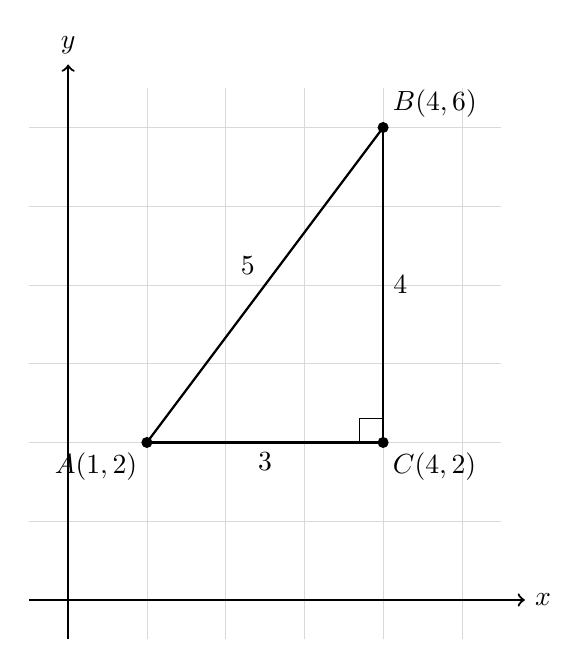
\begin{tikzpicture}[scale=1]
  \draw[step=1,gray!30,very thin] (-0.5,-0.5) grid (5.5,6.5);
  \draw[->,thick] (-0.5,0) -- (5.8,0) node[right] {$x$};
  \draw[->,thick] (0,-0.5) -- (0,6.8) node[above] {$y$};
  \fill (1,2) circle (2pt) node[below left] {$A(1,2)$};
  \fill (4,6) circle (2pt) node[above right] {$B(4,6)$};
  \fill (4,2) circle (2pt) node[below right] {$C(4,2)$};
  \draw[thick] (1,2) -- (4,2) node[midway,below] {$3$};
  \draw[thick] (4,2) -- (4,6) node[midway,right] {$4$};
  \draw[thick] (1,2) -- (4,6) node[midway,above left] {$5$};
  \draw (3.7,2) -- (3.7,2.3) -- (4,2.3);
\end{tikzpicture}
\end{center}

This formula deserves another look. On the left, $AB$ is a geometrical object---a segment's length. On the right is an algebraic object---arithmetic with coordinates and a square root. One formula, two languages: the first vehicle has crossed our coordinate bridge.

\begin{fanli}
``$A$ is at $(1,2)$ and $B$ at $(4,6)$. The horizontal difference is $3$ and the vertical difference $4$, so the distance is $3+4=7$.'' Wrong. $3+4$ is the length of a broken path that goes horizontally and then vertically, like a taxi following a grid of streets. The distance between two points means the straight segment, the diagonal shortcut. The Pythagorean theorem gives $\sqrt{3^{2}+4^{2}}=5$, which is indeed less than $7$, in agreement with the shortest-path property of a segment. Adding coordinate differences confuses road mileage with straight-line distance.
\end{fanli}

The distance formula has a useful by-product. What are the coordinates of the midpoint $M$ of $AB$? The intuitive answer is to average each pair of coordinates, and that intuition is correct:

\begin{tuilun}[The Midpoint Formula]
The midpoint $M$ of the segment joining $A(x_{1},y_{1})$ and $B(x_{2},y_{2})$ has coordinates
\[
M\left(\frac{x_{1}+x_{2}}{2},\ \frac{y_{1}+y_{2}}{2}\right).
\]
\end{tuilun}

Think of it this way: travelling from $A$ to $B$ changes the horizontal coordinate by $x_{2}-x_{1}$. Halfway along, the change is half as large, so the midpoint's horizontal coordinate is $x_{1}+\frac{x_{2}-x_{1}}{2}=\frac{x_{1}+x_{2}}{2}$. The vertical coordinate works the same way. For a rigorous proof, substitute the coordinates of $M$ into the distance formula and verify $AM=MB=\frac{1}{2}AB$; try it yourself. For example, the midpoint of $A(1,2)$ and $B(4,6)$ is $(\frac{5}{2},4)$, or $(2.5,4)$, which lies exactly halfway along the segment in the figure.

\section{An Equation Is a Shape's Identity Card}

So far, we have started with figures and calculated coordinates. Now reverse the direction and ask something more playful: \textbf{if we impose a rule on points in the plane, what shape do the obedient points form?}

For instance: ``the distance from the origin equals $3$.'' Your geometrical intuition may already shout, ``A circle!'' That is its definition. But pretend we do not know, and work through the coordinates. If an obedient point has coordinates $(x,y)$, the distance formula gives its distance from $(0,0)$, translating our rule into algebra:

\[
\sqrt{x^{2}+y^{2}}=3,\quad\text{squaring both sides gives}\quad x^{2}+y^{2}=9.
\]

A geometrical condition---fixed distance from a point---has become an algebraic equation, $x^{2}+y^{2}=9$. This equation acts like a sieve. Substitute $(3,0)$ and get $9+0=9$: it passes and lies on the circle. Substitute $(1,2)$ and get $1+4=5\ne 9$: it fails and lies off the circle. Substitute $(\sqrt{5},2)$ and get $5+4=9$: it lies on the circle. Every one of the countless points in the plane either passes or fails, and the passing points together form exactly the circle of radius $3$ centred at the origin, with no extras or omissions.

\begin{dingyi}[The Equation of a Curve and Its Locus]
If an equation $F(x,y)=0$ and a curve correspond in both directions---every point on the curve has coordinates satisfying the equation, and every point whose coordinates satisfy the equation lies on the curve---then the equation is called an equation of the curve, and the curve is called the graph (or locus) of the equation.
\end{dingyi}

A locus is an evocative idea: a point obeying a rule moves around the plane, and its trace is the locus. The rule written algebraically is an equation; the trace drawn geometrically is a curve. Here is a translation table:

\begin{center}
\begin{tabular}{ll}
\toprule
Algebra: equation & Geometry: figure \\
\midrule
$y=2x-1$ & A line (slope $2$, through $(0,-1)$) \\
$x^{2}+y^{2}=9$ & A circle of radius $3$ centred at the origin \\
$y=x^{2}$ & An upward-opening parabola with vertex at the origin \\
\bottomrule
\end{tabular}
\end{center}

You met the line in Chapter 2: the graph of a linear function $y=kx+b$ is a straight line. Now you have a new way to say it: the locus of the linear equation in two variables $y=kx+b$ is a line. The parabola is worth checking by hand. Set $x=0,\pm1,\pm2$ to obtain $y=0,1,1,4,4$, plot the five points, and join them with a smooth curve to get that famous bowl shape.

\begin{center}
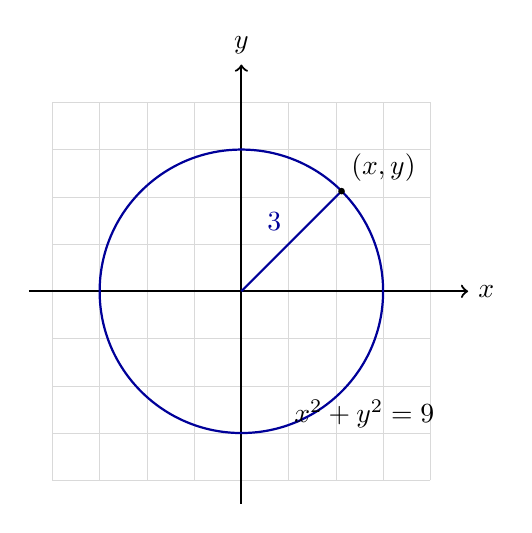
\begin{tikzpicture}[scale=0.6]
  \draw[step=1,gray!30,very thin] (-4,-4) grid (4,4);
  \draw[->,thick] (-4.5,0) -- (4.8,0) node[right] {$x$};
  \draw[->,thick] (0,-4.5) -- (0,4.8) node[above] {$y$};
  \draw[thick,blue!60!black] (0,0) circle (3);
  \draw[thick,blue!60!black] (0,0) -- (2.12,2.12) node[midway,above left] {$3$};
  \fill (2.12,2.12) circle (2pt) node[above right] {$(x,y)$};
  \node at (2.6,-2.6) {$x^{2}+y^{2}=9$};
\end{tikzpicture}
\hspace{8mm}
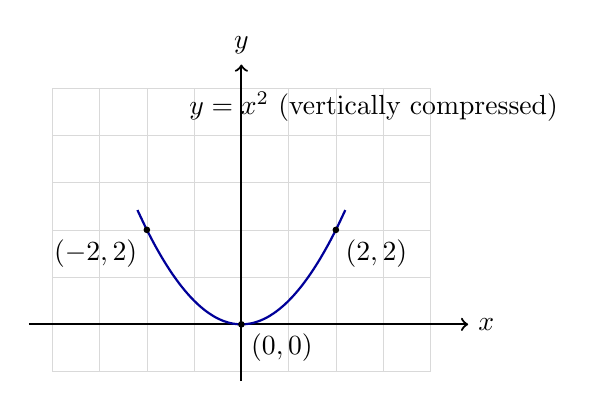
\begin{tikzpicture}[scale=0.6]
  \draw[step=1,gray!30,very thin] (-4,-1) grid (4,5);
  \draw[->,thick] (-4.5,0) -- (4.8,0) node[right] {$x$};
  \draw[->,thick] (0,-1.2) -- (0,5.5) node[above] {$y$};
  \draw[thick,blue!60!black,domain=-2.2:2.2,smooth] plot (\x,{0.5*\x*\x});
  \fill (0,0) circle (2pt) node[below right] {$(0,0)$};
  \fill (2,2) circle (2pt) node[below right] {$(2,2)$};
  \fill (-2,2) circle (2pt) node[below left] {$(-2,2)$};
  \node at (2.8,4.6) {$y=x^{2}$ (vertically compressed)};
\end{tikzpicture}
\end{center}

\begin{li}
Determine whether $P(2,\sqrt{5})$ lies on the circle $x^{2}+y^{2}=9$, and explain whether it lies inside or outside it.

Substitute into the left side: $2^{2}+(\sqrt{5})^{2}=4+5=9$, exactly the right side, so $P$ lies on the circle. Now consider $Q(1,1)$: $1^{2}+1^{2}=2<9$, so its distance from the origin is $\sqrt{2}$, less than the radius $3$, and it lies inside. In general, points with $x^{2}+y^{2}<9$ lie inside, and those with a value greater than $9$ lie outside. An equality identifies the curve, and two inequalities identify its two sides, all with the distance formula working behind the scenes.
\end{li}

\begin{shiyan}
Take coordinate paper, or draw a grid yourself, and mark $A(0,0)$ and $B(4,0)$. Look for points equidistant from $A$ and $B$. Start by measuring: $(2,0)$ is an obvious example; $(2,1)$ is $\sqrt{5}$ from both, so it also qualifies. What about $(2,3)$ and $(2,-2)$? Plot several such points and see what they form: a vertical line, precisely the perpendicular bisector of $AB$. Now verify it algebraically. If $(x,y)$ is equidistant from $A$ and $B$, then $\sqrt{x^{2}+y^{2}}=\sqrt{(x-4)^{2}+y^{2}}$. Squaring and simplifying gives $x^{2}=(x-4)^{2}$; expanding gives $8x=16$, or $x=2$. Geometry finds the perpendicular bisector by construction; algebra produces it in two lines of simplification.
\end{shiyan}

\section{Translation 1: Solving Geometry with Algebra}

Our bridge carries traffic both ways. First travel from geometry to algebra with a classic problem:

\textbf{Problem (the Triangle Midsegment Theorem)}: the segment joining the midpoints of two sides of a triangle is parallel to the third side and half its length.

In Chapter 3, the standard approach to such a problem was to add auxiliary lines and find congruent triangles. That takes some inspiration, which does not always arrive on time. Coordinates offer a route with a different temperament: patience is enough. Let us prove the theorem fully with coordinates.

Let the triangle's vertices be $A(x_{1},y_{1})$, $B(x_{2},y_{2})$, and $C(x_{3},y_{3})$. We deliberately avoid specific numbers because the theorem concerns \textbf{all} triangles; letters represent arbitrary choices.

Step 1: translate what is given. Let $M$ be the midpoint of $AB$ and $N$ the midpoint of $AC$. The midpoint formula gives

\[
M\left(\frac{x_{1}+x_{2}}{2},\frac{y_{1}+y_{2}}{2}\right),\qquad
N\left(\frac{x_{1}+x_{3}}{2},\frac{y_{1}+y_{3}}{2}\right).
\]

Step 2: translate the ``half'' part of the conclusion. Calculate $MN$ using the distance formula. The horizontal coordinate difference is

\[
\frac{x_{1}+x_{3}}{2}-\frac{x_{1}+x_{2}}{2}=\frac{x_{3}-x_{2}}{2},
\]

and the vertical difference is similarly $\frac{y_{3}-y_{2}}{2}$. Thus

\[
MN=\sqrt{\left(\frac{x_{3}-x_{2}}{2}\right)^{2}+\left(\frac{y_{3}-y_{2}}{2}\right)^{2}}
=\frac{1}{2}\sqrt{(x_{3}-x_{2})^{2}+(y_{3}-y_{2})^{2}}=\frac{1}{2}\,BC.
\]

We have proved the half-length claim. Every step merely combines fractions, extracts a factor of $\frac{1}{2}$, or applies the distance formula; none needs a flash of inspiration.

Step 3: translate ``parallel.'' What does parallelism mean in coordinates? Look at direction. From $M$ to $N$, the horizontal change is $\frac{x_{3}-x_{2}}{2}$ and the vertical change $\frac{y_{3}-y_{2}}{2}$. From $B$ to $C$, they are $x_{3}-x_{2}$ and $y_{3}-y_{2}$. Each change in the first journey is exactly half its counterpart in the second. The proportions of horizontal and vertical steps are identical, so the directions agree and $MN$ is parallel to $BC$. (If $x_{3}=x_{2}$, both horizontal changes are $0$, making both segments vertical and still parallel.) The theorem is proved.

Reflect on this method. A geometrical proof is like a detective, needing a flash of insight to discover the auxiliary line. A coordinate proof is like a mill: feed figures in to get coordinates, feed conclusions in to get equations, and grind steadily until a proof comes out. The mill is not romantic, but it never misses work. Coordinates also offer an advantage unavailable to the purely geometrical approach: \textbf{they handle whole batches}. Nearly the same routine works for many theorems, from the concurrence of three medians to diagonals bisecting one another. Algebra's spirit of solving a whole class of problems at once has crossed the bridge into geometry.

\section{Translation 2: Solving Algebra with Geometry}

Now send a vehicle in the other direction. Consider a problem that makes algebra frown:

\textbf{Problem}: for what value of $x$ does
\[
f(x)=\sqrt{x^{2}+9}+\sqrt{(6-x)^{2}+16}
\]
attain its minimum, and what is that minimum?

Pure algebra makes this awkward: two square roots enclose squares, completing the square does not finish the job, and squaring makes things more complicated. The algebraic tools available to a middle-school student are largely powerless. But after the previous section, a thought may occur: those radicals look remarkably like distance formulas.

The quantity $\sqrt{x^{2}+9}=\sqrt{(x-0)^{2}+(0-3)^{2}}$ measures the distance from $(x,0)$ to $(0,3)$. Likewise, $\sqrt{(6-x)^{2}+16}=\sqrt{(x-6)^{2}+(0-(-4))^{2}}$ measures the distance from $(x,0)$ to $(6,-4)$. So the expression says: choose $P(x,0)$ on the $x$-axis; its total distance to $A(0,3)$ and $B(6,-4)$ is $PA+PB$. Our problem becomes:

\textbf{The Translated Geometry Problem}: a point $P$ moves along the $x$-axis, with $A$ above the axis and $B$ below. Find the minimum of $PA+PB$.

Geometrically, the answer is almost immediate: a segment is the shortest path between two points. Since $A$ and $B$ lie on opposite sides of the $x$-axis, the segment joining $A$ and $B$ must cross the $x$-axis. Its intersection is the desired $P$. There, $PA+PB$ equals $AB$; at any other position of $P$, $PA+PB$ is a broken path and therefore longer. Thus the minimum is

\[
AB=\sqrt{(6-0)^{2}+(-4-3)^{2}}=\sqrt{36+49}=\sqrt{85}.
\]

$\sqrt{85}$ is approximately $9.22$. To find $x$ as well, follow $AB$ from $(0,3)$ to $(6,-4)$: it moves $6$ units horizontally while dropping $7$ vertically. Reaching the $x$-axis means dropping from $3$ to $0$, or $\frac{3}{7}$ of the total drop, so the horizontal journey is also $\frac{3}{7}$ of the total: $x=6\times\frac{3}{7}=\frac{18}{7}$. Substitute $x=\frac{18}{7}$ into the original expression to check that the two radicals sum to exactly $\sqrt{85}$.

Pause to appreciate what happened. We \textbf{did not calculate the algebraic expression directly}. We recognized its geometrical form and invoked a principle a three-year-old can understand: a straight path is shorter than a bent one. A forbidding algebraic minimum became an obvious geometrical fact. This is translation's second use: when one language obscures a problem, another may reveal its answer at once.

\begin{lianjie}
This kind of translation is no armchair game. Navigation software performs this chapter's demonstrations constantly: satellites supply latitude and longitude (coordinates), streets become lines in a plane, and the shortest route becomes a problem about distances and broken paths. A game character jumps along a parabola because a program repeatedly evaluates equations like $y=x^{2}$. A doctor's CT image is essentially a machine reconstructing a picture from numerical density information at points in a cross-section. Looking across the book, Chapter 2's function graphs first introduced equations becoming curves, and this chapter made that a systematic method. Chapter 7's vectors will turn translations and rotations of points into algebra too. And calculus's central activity---studying the bending and changing of curves---rests at every step on this coordinate bridge.
\end{lianjie}

\section{Setting Points in Motion: Parametric Equations}

So far, equations describe static pictures: which points lie on a curve and which do not. But real-world points are almost always moving: a second hand's tip circles a clock, a thrown basketball traces an arc, and a game character runs across a screen. How can we write an equation for motion itself?

Look again at our old friend, the parabola $y=x^{2}$. Imagine it as the trail of a crawling ball. The ball starts at the origin, moves rightward at $1$ unit per second, and changes height according to a time rule. If $t$ is the number of seconds since departure, then

\[
x=t,\qquad y=t^{2}.
\]

At $t=0$ the ball is at $(0,0)$; at $t=1$, at $(1,1)$; at $t=2$, at $(2,4)$; and at $t=3$, at $(3,9)$. At each second it has a definite position, and together the positions trace the same parabola. See the difference? $y=x^{2}$ describes the relationship between the coordinates, without saying when the point arrives. The pair $x=t$, $y=t^{2}$ tells us where it is at each moment: it draws the route and records a timetable. The extra variable $t$ is a \textbf{parameter}, and the pair forms \textbf{parametric equations}.

\begin{dingyi}[Parametric Equations]
Suppose the coordinates $(x,y)$ of a point moving on a curve are expressed in terms of a variable $t$ as
\[
x=f(t),\qquad y=g(t),
\]
and as $t$ ranges over its allowed values, $(x,y)$ traces exactly the curve. Then these are parametric equations of the curve, and $t$ is the parameter.
\end{dingyi}

A parameter often plays the role of time, but it need not be time: it is simply a conductor's baton---as $t$ changes, the point moves. Here is a more physical example. Throw a ball horizontally, neglecting air resistance; it moves rightward at constant speed and accelerates downward. Simplifying the numbers rather than using precise gravitational data, write

\[
x=2t,\qquad y=5-t^{2}\quad(t\ge 0).
\]

At $t=0$ the ball is at $(0,5)$, released at height $5$; at $t=1$, at $(2,4)$; and at $t=2$, at $(4,1)$. For slightly larger $t$, $y$ becomes negative and the ball has reached the ground. If we care only about the arc's shape and not the timing, we can \textbf{eliminate} the parameter. The first equation gives $t=\frac{x}{2}$; substitute into the second:

\[
y=5-\left(\frac{x}{2}\right)^{2}=5-\frac{x^{2}}{4}.
\]

The parameter disappears, leaving a downward-opening parabola. Horizontal projectile motion indeed traces a parabola, in the same family as a basketball shot or a fountain's stream. Eliminating $t$ returns us to an ordinary equation. Conversely, one curve can have many parametric descriptions, representing different ways to travel the same route. $x=t$, $y=t^{2}$ climbs the parabola with constant horizontal speed; $x=t^{3}$, $y=t^{6}$ traces the same right-hand arc at a different pace. The locus is the stage and the parametric equations the script: one stage can host many scripts.

Why set points in motion? Because so many questions naturally involve time or progress: when a planet comes closest to the Sun, where a shell lands, or which screen pixel should hold a character in this animation frame. A static equation says which road a point is on; parametric equations say where on that road it is now. The latter is much closer to what engineers and physicists actually want to ask.

\begin{pandeng}
Beyond the coordinate bridge lies a vast continent. Its landmarks include \textbf{analytic geometry}, the systematic study of translating between equations and curves, whose founders are generally recognized as Descartes and Fermat, reportedly rivals over priority; \textbf{conic sections}, asking why ellipses, parabolas, and hyperbolas are called conics and how they relate to planetary orbits; \textbf{polar coordinates}, which address points using distance and direction, as on a radar screen; and \textbf{parametric equations and calculus}, asking how a timetable $x=f(t)$, $y=g(t)$ reveals velocity at each instant. It is fine if these names are unfamiliar: think of them as regions of the map yet to be unlocked.
\end{pandeng}

\begin{toolbox}
This chapter's new tools, in order of appearance:

\begin{itemize}
\item \textbf{The number line and one-to-one correspondence}: real numbers correspond one to one with points on a line; one-dimensional distance $=\lvert b-a\rvert$.
\item \textbf{Cartesian coordinates in the plane}: points correspond one to one with ordered pairs $(x,y)$; order matters.
\item \textbf{The distance formula}: $AB=\sqrt{(x_{2}-x_{1})^{2}+(y_{2}-y_{1})^{2}}$, essentially the Pythagorean theorem in coordinates.
\item \textbf{The midpoint formula}: midpoint coordinates are the averages of the endpoint coordinates.
\item \textbf{Translating equations and loci}: a point lies on a curve if and only if its coordinates satisfy the equation; a geometrical condition produces an equation, and an equation traces a curve.
\item \textbf{Solving in both directions}: coordinates let us calculate geometry problems directly; algebra problems, especially those with radicals, can become distances that we recognize geometrically.
\item \textbf{Parametric equations}: a third variable $t$ records a moving point's timetable; eliminating the parameter restores an ordinary equation.
\end{itemize}
\end{toolbox}

\section*{Questions to Think About}

\textbf{Observation}

\begin{sikao}
\item Set $t=-2,-1,0,1,2$ in the parametric equations $x=t^{2}$, $y=2t$, plot the resulting points, and join them smoothly. What shape do you see? Hint: solve the second equation for $t=\frac{y}{2}$, substitute into the first to eliminate $t$, and examine the equation relating $x$ and $y$. How is it related to $y=x^{2}$?
\item On coordinate paper, shade the region satisfying $x^{2}+y^{2}\le 9$, then mark the region satisfying $x+y>0$ in a different way. What does their overlap look like? Hint: first draw the boundaries $x^{2}+y^{2}=9$ and $x+y=0$. To identify the appropriate side of a boundary, substitute a test point, such as the origin.
\end{sikao}

\textbf{Proof}

\begin{sikao}
\item Use coordinates to prove that a quadrilateral whose diagonals bisect each other is a parallelogram. Hint: put the common midpoint at the origin, one pair of opposite vertices at $(a,b)$ and $(-a,-b)$, and the other pair at $(c,d)$ and $(-c,-d)$. Compare the horizontal and vertical steps along each pair of opposite sides.
\item Two fixed points are $A(-1,0)$ and $B(1,0)$. A moving point $P(x,y)$ satisfies $PA^{2}+PB^{2}=10$. Prove that the locus of $P$ is a circle, and identify its centre and radius. Hint: expand $PA^{2}$ and $PB^{2}$ using the distance formula (these are \textbf{squared} distances, so the radicals disappear), combine like terms, and inspect the result.
\end{sikao}

\textbf{Challenge}

\begin{sikao}
\item Find the minimum of $\sqrt{x^{2}-2x+2}+\sqrt{x^{2}-8x+20}$. Hint: complete the square inside each radical and recognize two distances. This time the fixed points lie on the same side of the $x$-axis, so joining them directly will not work. Think of a mirror: reflect one point across the $x$-axis. The broken path keeps its length, and a straight line can now help.
\item A point $P$ moves along $y=x^{2}$ and can be written $(t,t^{2})$; a fixed point $A$ is $(2,0)$. Express $PA^{2}$ in terms of $t$. Hint: apply the distance formula but do not rush to take a square root. $PA^{2}$ is a \textbf{quartic} expression in $t$. Middle-school completion of squares no longer reveals whether it has a minimum or where it occurs. This puzzling quartic is exactly the sort of object the next chapter will investigate.
\end{sikao}

\section*{The Door to the Next Chapter}

With the bridge open, one of the first pieces of cargo across the river is a curve we have met repeatedly: the parabola.

Draw $y=x^{2}-3x+2$ on coordinate paper, and it meets the $x$-axis twice. At each meeting the vertical coordinate is $0$, so the horizontal coordinate must satisfy $x^{2}-3x+2=0$, a quadratic equation. In other words, \textbf{intersections with the $x$-axis and roots of an equation are two descriptions of the same thing}: geometry sees them, and algebra calculates them. The equation $x^{2}-3x+2=0$ has roots $1$ and $2$, so the parabola meets the $x$-axis exactly at $(1,0)$ and $(2,0)$.

A stream of new questions now crosses the bridge. Replace degree $2$ with degree $3$: how many times does $y=x^{3}-x$ meet the $x$-axis? What about degrees $4$ and $5$? Can a polynomial curve never meet the $x$-axis---can an equation have no real roots at all? If so, is the problem wrong, or is our world of numbers too small and ready for expansion?

The common protagonists are expressions like $x^{2}-3x+2$ and $x^{3}-x$, assembled by adding and subtracting powers of letters: \textbf{polynomials}. They seem like simple algebraic components, but they hide roots of equations, intersections of curves, and even clues to the birth of a new number system. At our next stop, we will take polynomials apart and examine their structure.
